\documentclass[utf8]{beamer}

\mode<presentation>
{
  \usetheme{Warsaw}
  \setbeamercovered{transparent}
}


\usepackage{amsfonts,mathtools,amssymb}
\usepackage[spanish]{babel}
\usepackage{times}
\usepackage[T1]{fontenc}
\usepackage[shortlabels]{enumitem}
\usepackage{tikz}
\usepackage{physics}

\title[MA0505]{MA0505 - An\'alisis I}
\subtitle{Lecci\'on XII: La Medida Exterior}

\author{Pedro M\'endez\inst{1}}

\institute[Universidad de Costa Rica] % (optional, but mostly needed)
{
  \inst{1}%
  Departmento de Matem\'atica Pura y Ciencias Actuariales\\
  Universidad de Costa Rica
  }

\date[I-2021] {Semestre I, 2021}

%%%%%%%%% === Theorems and suchlike === %%%%%%%%%%%%%%

\theoremstyle{plain}
\newtheorem{Th}{Teorema}               %%% Theorem 1.1.1
\newtheorem{Tmon}{Teoremón}
\newtheorem{Prop}{Proposición}         %%% Proposition 1.1.2
\newtheorem{Lem}{Lema}                 %%% Lemma 3
\newtheorem{Cor}{Corolario}            %%% Corollary 4

\theoremstyle{definition}
\newtheorem{Def}{Definición}           %%% Definition 5
\newtheorem{Ex}{Ejemplo}               %%% Example 6
\newtheorem{Ej}{Ejercicio}             %%% Ejercicio 7
\newtheorem{Hec}[Th]{Hecho}            %%% Hecho 1.1.8

\theoremstyle{remark}
\newtheorem{Rmk}[Th]{Observación}      %%%Remark 1.1.9
\newtheorem*{nonum-Rmk}{Observación}         %%% No number Fact
\newtheorem*{Notn}{Notaci\'on}        %% Notaciones
\newtheorem*{Warn}{Advertencia}       %% Advertencias

\numberwithin{equation}{section}

%% Accomodations 

\makeatletter
\def\moverlay{\mathpalette\mov@rlay}
\def\mov@rlay#1#2{\leavevmode\vtop{%
   \baselineskip\z@skip \lineskiplimit-\maxdimen
   \ialign{\hfil$\m@th#1##$\hfil\cr#2\crcr}}}
\newcommand{\charfusion}[3][\mathord]{
    #1{\ifx#1\mathop\vphantom{#2}\fi
        \mathpalette\mov@rlay{#2\cr#3}
      }
    \ifx#1\mathop\expandafter\displaylimits\fi}
\makeatother

% Greek letters:

\newcommand{\al}{\alpha}                %% short for  \alpha
\newcommand{\bt}{\beta}                 %% short for  \beta
\newcommand{\Dl}{\Delta}                %% short for  \Delta
\newcommand{\dl}{\delta}                %% short for  \delta
\newcommand{\eps}{\varepsilon}          %% short for  \varepsilon
\newcommand{\Ga}{\Gamma}                %% short for  \Gamma
\newcommand{\ga}{\gamma}                %% short for  \gamma
\newcommand{\La}{\Lambda}               %% short for  \Lambda
\newcommand{\la}{\lambda}               %% short for  \lambda
\newcommand{\Om}{\Omega}                %% short for  \Omega
\newcommand{\om}{\omega}                %% short for  \omega
\newcommand{\Sg}{\Sigma}                %% short for  \Sigma
\newcommand{\sg}{\sigma}                %% short for  \sigma
\newcommand{\te}{\theta}                %% short for  \theta
\newcommand{\vf}{\varphi}               %% short for  \varphi
\newcommand{\ze}{\zeta}                 %% short for  \zeta

%Boldface letters

\newcommand{\bC}{\mathbb{C}}    %%% números complejos
\newcommand{\bN}{\mathbb{N}}    %%% números naturales
\newcommand{\bP}{\mathbb{P}}        %% números enteros positivos
\newcommand{\bQ}{\mathbb{Q}}    %%% números racionales
\newcommand{\bR}{\mathbb{R}}    %%% números reales
\newcommand{\bS}{\mathbb{S}}    %%% esfera
\newcommand{\bZ}{\mathbb{Z}}    %%% números enteros

%Script letters:

\newcommand{\cA}{\mathcal{A}}           %% formas diferenciales
\newcommand{\cB}{\mathcal{B}}           %% una base vectorial
\newcommand{\cC}{\mathcal{C}}           %% otra base vectorial
\newcommand{\cF}{\mathcal{F}}           %% espacio de Fock
\newcommand{\cL}{\mathcal{L}}           %% operadores lineales
\newcommand{\cM}{\mathcal{M}}           %% multiplicadores
\newcommand{\cN}{\mathcal{N}}           %% funciones nulas
\newcommand{\cP}{\mathcal{P}}           %% una particion
\newcommand{\cR}{\mathcal{R}}           %% funciones representativas
\newcommand{\cS}{\mathcal{S}}           %% funciones de Schwartz


%Brackets

\newcommand{\bonj}[1]{\left\lbrack#1\right\rbrack}
\newcommand{\obonj}[1]{\left\rbrack#1\right\lbrack}
\newcommand{\rbonj}[1]{\left\rbrack#1\right\rbrack}
\newcommand{\lbonj}[1]{\left\lbrack#1\right\lbrack}
\newcommand{\snm}[1]{\|#1\|}           %small norma
\newcommand{\nm}[1]{\left\|#1\right\|} %norma pegadita
\newcommand{\pnm}[1]{\biggl|\biggl|#1\biggr|\biggr|}
\newcommand{\set}[1]{\{\,#1\,\}}    %% set notation
\newcommand{\floor}[1]{\lfloor#1\rfloor} %% mayor entero <= x
\newcommand{\Set}[1]{\biggl\{\,#1\,\biggr\}} %% set notation (large)
\newcommand\quot[2]{
        \mathchoice
            {% \displaystyle
                \text{\raise1ex\hbox{$#1$}\Big/\lower1ex\hbox{$#2$}}%
            }
            {% \textstyle
                {^{ #1}/_{ #2}}
            }
            {% \scriptstyle
                {^{ #1}/_{ #2}}
            }
            {% \scriptscriptstyle
                {^{ #1}/_{ #2}}
            }
    }
\newcommand*\squot[2]{{^{ #1}/_{ #2}}}%%%small quotient

%Symbols 

\newcommand{\x}{\times}
\renewcommand{\geq}{\geqslant}          %% mayor o igual (variante)
\newcommand{\hookto}{\hookrightarrow}     %% inclusion arrow
\newcommand{\isom}{\simeq}              %% isomorfismo
\renewcommand{\l}{\ell}                   %% ele cursiva
\renewcommand{\leq}{\leqslant}          %% menor o igual (variante)
\newcommand{\less}{\setminus}           %% set difference
\newcommand{\To}{\Rightarrow}
\newcommand{\ov}{\overline}
\newcommand{\un}{\underline}
\newcommand{\del}{\partial}
\newcommand{\ind}{\mathbf{1}}       %%%indicator function

%%% Small fractions in displays:

\newcommand{\half}{{\mathchoice{\nhalf}{\thalf}{\shalf}{\shalf}}} %%display text script script^2
\newcommand{\happi}{{\tfrac{\pi}{2}}} %% small fraction  \pi/2
\newcommand{\quarter}{\tfrac{1}{4}} %% small fraction  1/4
\newcommand{\nhalf}{\frac{1}{2}}
\newcommand{\shalf}{{\scriptstyle\frac{1}{2}}} %% tiny fraction 1/2
\newcommand{\thalf}{{\tfrac{1}{2}}} %% small fraction  1/2
\newcommand{\third}{\tfrac{1}{3}}   %% small fraction  1/3 %Hay que renew porque mathabx toma second y third como x'' y x''' por ejemplo

\newcommand{\ihalf}{{\tfrac{i}{2}}} %% small fraction  i/2

\newcommand{\suci}{_{i=1}^\infty} %% diminutivo
\newcommand{\suck}{_{k=1}^\infty} %% diminutivo
\newcommand{\sucl}{_{\l=1}^\infty} %% diminutivo
\newcommand{\sucm}{_{m=1}^\infty} %% diminutivo
\newcommand{\sucn}{_{n=1}^\infty} %% diminutivo

\newcommand*{\Cdot}{{\raisebox{-0.25ex}{\scalebox{1.5}{$\cdot$}}}}      %% cdot más grande
\renewcommand{\.}{\Cdot}                %% producto escalar
\newcommand{\cupdot}{\charfusion[\mathbin]{\cup}{\.}}
\newcommand{\bigcupdot}{\charfusion[\mathbin]{\bigcup}{\.}}
\DeclareMathOperator{\Var}{Var}     %%%variance

\begin{document}

\begin{frame}
  \titlepage
\end{frame}

\begin{frame}{Agenda}
  \tableofcontents
  % You might wish to add the option [pausesections]
\end{frame}


% Structuring a talk is a difficult task and the following structure
% may not be suitable. Here are some rules that apply for this
% solution: 

% - Exactly two or three sections (other than the summary).
% - At *most* three subsections per section.
% - Talk about 30s to 2min per frame. So there should be between about
%   15 and 30 frames, all told.

% - A conference audience is likely to know very little of what you
%   are going to talk about. So *simplify*!
% - In a 20min talk, getting the main ideas across is hard
%   enough. Leave out details, even if it means being less precise than
%   you think necessary.
% - If you omit details that are vital to the proof/implementation,
%   just say so once. Everybody will be happy with that.

\section{Motivación}

\begin{frame}{La Longitud de un segmento}
  Considere el segmento 
  \begin{figure}
    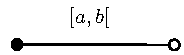
\includegraphics{figs/1/fig1.pdf}
  \end{figure}
  La longitud del segmento es 
  $$b-a=\text{longitud}([a,b[)=\l([a,b[).$$
  Si tenemos intervalos disjuntos
  \begin{figure}
    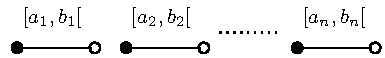
\includegraphics{figs/2/fig2.pdf}
  \end{figure}
  Entonces su longitud es $\sum_{i=1}^nb_i-a_i$.
\end{frame}

\begin{frame}{¿Cuál es la Longitud de un Punto?}
  Si tenemos $\set{a}\subseteq[a,a+\eps[$, entonces 
  $$\l(a)\leq \eps$$
  para $\eps>0$. De manera que la longitud del punto es cero.
\end{frame}

\begin{frame}{Los Racionales}
  Sea $\bQ\cap[0,1]=\set{q_n}\sucn$, entonces
  $$\l\left(\bigcup_{i=1}^n\set{q_i}\right)=\sum_{i=1}^n\l(\set{q_i})=0.$$
  Entonces, ¿cuál es la longitud de $\bQ\cap[0,1]$? Note que $\displaystyle\int_a^b\dd x=b-a$. 
\end{frame}

\begin{frame}{Unas Observaciones}
  De hecho si $[a,b[\subseteq[0,1]$, entonces
  \begin{enumerate}[(i)]
    \item $\displaystyle b-a=\int\limits_0^1\ind_{\lbonj{a,b}}(x)\dd x$.
    \item $\displaystyle \sum_{i=1}^nb_i-a_i=\int\limits_0^1\sum_{i=1}^n\ind_{\lbonj{a_i,b_i}}(x)\dd x=\int\limits_0^1\ind_{\bigcup_{i=1}^n\lbonj{a_i,b_i}}(x)\dd x$.
    \item $\displaystyle 0=\int\limits_0^1\ind_{\set{a}}(x)\dd x$.
  \end{enumerate}
\end{frame}

\begin{frame}{Volviendo a la Pregunta}
  En este caso $\displaystyle\int\limits_0^1\ind_{\bigcup_{i=1}^n\set{q_i}}(x)\dd x=0$. Note que $\ind_{\lbonj{0,1}\cap\bQ}=\lim_{n\to\infty}\ind_{\bigcup_{i=1}^n\set{q_i}}$.\par 
  Luego si $\ind_{\lbonj{0,1}\cap\bQ}$ fuese integrable y se pudieren tomar límites, tenemos que 
  $$\int\limits_0^1\ind_{\bQ\cap\bonj{0,1}}(x)\dd x=\lim_{n\to\infty}\int\limits_0^1\ind_{\bigcup_{i=1}^n\set{q_i}}(x)\dd x=0.$$
  ¿Qué integral estamos usando? Recordemos que $\ind_{\bQ\cap\bonj{0,1}}$ no es Riemann integrable.
\end{frame}

\section{Definición de Medida Exterior}

\subsection{Medida en Dimensión 1}
\begin{frame}
  Consideremos las familias
  \begin{itemize}
    \item $\displaystyle S=\set{\lbonj{a,b}:\ a<b}\cup\set{\rbonj{-\infty,b}:\ b\in\bR}\cup\set{\lbonj{a,\infty}:\ a\in\bR}\cup \emptyset$.
    \item $\displaystyle\cS_1=\Set{\bigcup_{i=1}^n I_i;\ I_i\in S,\ 1\leq i\leq n}$.
  \end{itemize}
Note que $[a,b]\not\in\cS_1$, pero $\bR=\lbonj{-\infty,b}\cup\rbonj{b,\infty}\in\cS_1$. Por lo tanto, dado $A\subseteq\bR$, existe $B\in\cS_1$ tal que $A\subseteq B$.
\end{frame}

\begin{frame}{La Definición}\label{fr:unaPrimeraDefn}
  Definimos $m:\cS_1\to\bR$ por:
  \begin{enumerate}
    \item $m(\bonj{a,b})=b-a$ si $a<b$.
    \item $m(\lbonj{a,\infty})=m(\rbonj{-\infty,b})=\infty$.
    \item $m\left(\bigcup_{i=1}^k I_i\right)=\sum_{i=1}^kb_i-a_i$ para $I_i=[a_i,b_i]$ que satisface $\obonj{a_i,b_i}\cap\obonj{a_j,b_j}=\emptyset$ si $i\neq j$.
  \end{enumerate}
\end{frame}

\begin{frame}{¿Está bien definida?}
  Por ejemplo
  \begin{figure}
    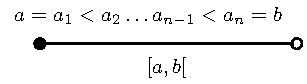
\includegraphics{figs/3/fig3.pdf}
  \end{figure}
  Vale $[a,b]=\bigcup_{i=1}^{n-1}[a_i,a_{i+1}]$, con $\obonj{a_j,a_{j+1}}\cap\obonj{a_i,a_{i+1}}=d$ cuando $i\neq j$. Entonces 
 $$m^\ast\left(\bigcup_{i=1}^{n-1}[a_i,a_{i+1}]\right)=\sum_{i=1}^{n-1}a_{i+1}-a_i=b-a.$$
  \begin{figure}
    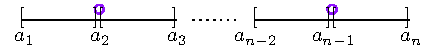
\includegraphics{figs/4/fig4.pdf}
  \end{figure}
\end{frame}

\begin{frame}
  Note que si 
  $$[a,b]\subseteq [a_1,b_1]\cup[a_2,b_2]$$
  pero $\obonj{a_1,b_1}\cap \obonj{a_2,b_2}\neq\emptyset$, entonces $a_2<b_1$
  $$\To b_2-a_2+b_1-a_1>b-a=b_2-a_1.$$
  \begin{Ej}\label{ej:medidasYSumas}
Si $\bigcup_{k=1}^nI_k=\bigcup_{\l=1}^mJ_\l$ son tales que $I_k^o\cap I^o_\l$, entonces %La condición es correcta?
$$\sum_{k=1}^nm(I_k)\leq \sum_{\l=1}^mm(J_\l).$$
  \end{Ej}
\end{frame}

\begin{frame}{¿Cómo Medimos Otros Conjuntos?}
  \begin{Def}\label{def:medidaExterior}
    Dado $E\subseteq\bR$, definimos su \alert{medida exterior} como
    $$m_e(E)=\inf\Set{\sum\suck m(I_k):\ E\subseteq\bigcup\suck I_k,\ I_k\in S}.$$ %whois S
  \end{Def}
  Note que, si $E_1\subseteq E_2$, entonces $m_e(E_1)\leq m_e(E_2)$. 
  \begin{Lem}\label{lem:medidaUnIntervalo}
    Sea $E=[a,b]$. Entonces $m_e(E)=b-a$.
  \end{Lem}
\end{frame}

\begin{frame}{Prueba del Lema}
  \begin{itemize}
    \item Dado que $[a,b]\in S$, tenemos que $m_e([a,b])\leq b-a$. 
    \item Sean $I_k\in S$ tales que $[a,b]\subseteq\bigcup\suck I_k$.
    \item Si los intervalos fueran abiertos, podemos reducir la unión a una unión finita.
    \item Sean $I_k^\ast=\obonj{c_k,d_k}$ tales que $I_k\subseteq I_k^\ast$ y $m(\ov I_k)\leq(1+\eps)m(I_k)$. 
    \item Note que $[a,b]\subseteq\bigcup\suck I_k^\ast$ y por compacidad, existe un $k_0$ tal que 
    $$[a,b]\subseteq \bigcup_{k=1}^{k_0}I_k^\ast\subseteq\bigcup_{k=1}^{k_0}\ov {I_k^\ast}.$$
  \end{itemize}
\end{frame}

\begin{frame}{Terminamos la Prueba}
  Entonces vale
  $$b-a\leq\sum_{k=1}^{k_0}m(\ov {I_k^\ast})\leq(1+\eps)\sum_{k=1}^{k_0}m(I_k)\leq (1+\eps)\sum\suck m(I_k).$$
  Por lo tanto 
  $$\frac{b-a}{1+\eps}\leq \sum\suck m(I_k)\To\frac{b-a}{1+\eps}\leq m_e([a,b]).$$
\end{frame}

\begin{frame}{Subaditividad}
  \begin{Lem}\label{lem:subadivitidad}
Sean $E\subseteq \bR$ y $E_i\subseteq\bR$ para $i\geq 1$. Si $E=\bigcup\suck E_k$, entonces
$$m_e(E)\leq\sum\suck m_e(E_k).$$
  \end{Lem}
  Sin perdida de generalidad, supongamos que $m(E_k)<\infty$. Luego, existen $\set{I_i^k}\suci$ tales que $I_i^k\in S$ y 
  $$m_e(E_k)\leq \sum\suci m(I_i^k)\leq m_e(E_k)+\frac{\eps}{2^k}.$$
\end{frame}

\begin{frame}{Terminamos la Prueba}
  Como $E\subseteq \bigcup\suck\bigcup\suci I_i^k$, concluimos que 
\begin{align*}
  m_e(E)&\leq \sum\suck\sum\suci m(I_i^k)\\
  &\leq \sum\suck m_e(E_k)+\underbrace{\sum\suck \frac{\eps}{2^k}}_{\eps}.
\end{align*}
\end{frame}

\subsection{Medida en Dimensión Mayor}

\begin{frame}{Generalización}
  Estos resultados se pueden generalizar a varias dimensiones. Dado 
  $$S_d=\set{[a_1,b_1]\x\dots\x[a_d,b_d]:\ a_k\leq b_k,\ 1\leq k\leq d}$$
  y $E\subseteq\bR^d$, definimos 
  $$m_e(E)=\inf\Set{\sum\suck m(I_k):\ E\subseteq \bigcup\suck I_k,\ I_k\in S_d}.$$
 
\end{frame}

\begin{frame}{Resultados Análogos}
  De forma similar se pueden probar los siguientes resultados.
  \begin{Lem}\label{lem:medidaCajaDDim}
    Sea $I=[a_1,b_1]\x\dots\x[a_d,b_d]$, entonces $m_e(I)=\prod_{k=1}^d(b_k-a_k)$.
  \end{Lem}
  \begin{Lem}\label{lem:subaditividadEnDDim}
    Sean $E_i\subseteq\bR^d$ para $i\geq 1$. Entonces 
    $$m_e\left(\bigcup\suci E_i\right)\leq\sum\suci m_e(E_i).$$
  \end{Lem}
\end{frame}

\begin{frame}{Ejemplos}
  \begin{enumerate}[a)]
    \item Si $m_e(E_i)=0$ para $i\geq 1$, entonces
    $$m_e\left(\bigcup\suci E_i\right)\leq \sum\suci m_e(E_i)=0.$$
    \item Sea $x=(x_1,\dots,x_d)$, entonces $\set{x}\subseteq[x_1,x_1+\eps]\x\dots[x_d,x_d+\eps]$. Así $m_e(\set{x})\leq \eps^d$ y por lo tanto $m_e(\set{x})=0$.
    \item Del anterior se sigue que $m_e(\bQ)=0$.
  \end{enumerate}
\end{frame}

\begin{frame}{Un Lema Muy Útil}
  La medida exterior se puede aproximar utilizando abiertos.
  \begin{Lem}\label{lem:aproxConAbiertos}
    Sean $E\subseteq\bR^d$ y $\eps>0$, entonces existe $G\subseteq\bR^d$ tal que $E\subseteq G$ y 
    $$m_e(E)\leq m_e(G)\leq m_e(E)+\eps.$$
  \end{Lem}
  Este resultado garantiza la existencia de $G$, un abierto, tal que $E\subseteq G$ y $m_e(E)=m_e(G)$.
\end{frame}

\begin{frame}
\begin{Def}\label{def:Gdelta}
  Un conjunto $H\subseteq\bR^d$ se dice ser \alert{$G_\dl$} si existen $G_k$, $k\geq 1$, abiertos tales que $H=\bigcap\suck G_k$.
\end{Def}  
\begin{Lem}\label{lem:GdelApprox}
  Sea $E\subseteq\bR^d$, entonces existe $E\subseteq H$, un conjunto $G_\dl$ tal que $m_e(E)=m_e(H)$.
\end{Lem}

\end{frame}
\begin{frame}{Prueba del Lema}
  En efecto, para $k\geq 1$, existe $G_k$ tal que $E\subseteq G_k$ y 
$$m_e(E)\leq m_e(G_k)\leq m_e(E)+\frac1k.$$
Considere $H=\bigcap\suck G_k$, entonces $E\subseteq H$ y además 
$$m_e(H)\leq m_e(E)+\frac1k$$
para $k\geq 1$. Por lo tanto $m_e(H)=m_e(E)$.
\end{frame}

\section{La Medida de Lebesgue}

\begin{frame}
  \begin{Def}\label{def:LebesgueMedible}
    Llamamos a $E\subseteq\bR^d$ \alert{Lebesgue medible} si para $\eps>0$, existe $G$ abierto tal que $E\subseteq G$ y $m_e(G\less E)<\eps$.\par 
    Si $E$ es (Lebesgue) medible, definimos su medida de Lebesgue como $m(E)=m_e(E)$.
  \end{Def}
  
\end{frame}
\subsection{Conjuntos Medibles}
\begin{frame}{Un Par de Ejemplos}
  \begin{enumerate}[a)]
  \item Por ejemplo si $E=[a,b]$, entonces $E\subseteq\obonj{a-\eps,b+\eps}$. Entonces
    $$m_e(G\less E)=m_e(\obonj{a-\eps,a}\cup\obonj{b,b+\eps})\leq 2\eps.$$
    En general $\lbonj{a,b},\rbonj{a,b}$ y $\obonj{a,b}$ son medibles y $m(\bonj{a,b})=b-a$.
   \item Si tenemos $E$ tal que $m_e(E)=0$, entonces existe $G$ un abierto tal que $E\subseteq G$ y 
    $$m_e(E)\leq m_e(G)<\eps.$$
    Luego 
    $$m_e(G\less E)\leq m_e(G)<\eps.$$
\end{enumerate}
\end{frame}

\begin{frame}{Uniones}
  \begin{Th}\label{thm:unionDeMedibles}
  Sea $\set{E_i}\suci$ una familia de conjuntos medibles. Entonces $\bigcup\suci E_i$ es medible.
  \end{Th}
  
\end{frame}

\begin{frame}
  \begin{itemize}
    \item Sea $\eps>0$, entonces existen $G_i$ abiertos tales que $E_i\subseteq G_i$ y $m_e(G_i\less E_i)<\frac{\eps}{2^i}$. 
    \item Luego, $G=\bigcup\suci G_i$ es abierto y 
     $$G\less E=\bigcup\suci G_i\less E\subseteq \bigcup\suci G_i\less E_i.$$
     \item Se sigue que 
     $$m_e(G\less E)\leq \sum\suci m_e(G_i\less E_i)<\sum\suci\frac{\eps}{2^i}=\eps.$$
  \end{itemize}
\end{frame}

\begin{frame}{La Unión de Cajas}
  \begin{Th}\label{thm:UnionDeCajas}
    Sea $I_k=I_1^k\x\dots\x I_d^k$ con $I_i^k$ un intervalo finito. Si $I_i^o\cap I_j^o=\emptyset$, entonces 
    $$m_e\left(\bigcup_{j=1}^mI_j\right)=\sum_{j=1}^mm_e(I_j).$$  
  \end{Th}
  \begin{Ej}
    Pruebe el teorema anterior.
  \end{Ej}
\end{frame}

\begin{frame}
  \begin{Lem}\label{lem:ADistPositiva}
    Si $d(E_1,E_2)>0$ entonces 
    $$m_e(E_1\cup E_2)=m_e(E_1)+m_e(E_2).$$
  \end{Lem}
  Tomemos $\eps>0$ y $\bigcup\suck I_k$ tal que 
  $$\sum\suck m(I_k)\leq \eps+m_e(E_1\cup E_2).$$
  Sin perdida de generalidad asumimos que 
  $$\text{diam}(I_k)\leq\half d(E_1,E_2)$$
\end{frame}

\begin{frame}
  Note que si $E_1\cap I_k\neq \emptyset$, entonces $E_2\cap I_k=\emptyset$. Luego 

   $$E_1\subseteq \bigcup_{\substack{k=1\\ I_k\cap E_1\neq\emptyset}}^\infty I_k=\bigcup\sucl J_\l,\quad E_2\subseteq \bigcup_{\substack{k=1\\ I_k\cap E_2\neq\emptyset}}^\infty I_k=\bigcup\sucl \tilde J_\l.$$

  De aquí que 
 $$m_e(E_1)\leq\sum\sucl m(J_\l),\quad m_e(E_2)\leq \sum\sucl m(\tilde{J}_\l).$$
 Por lo tanto 
 $$m_e(E_1)+m_e(E_2)\leq sum\suck m(I_k)\leq m_e(E_1\cup E_2)+\eps.$$ 
\end{frame}
\section*{Resumen}

\subsection*{Qu\'e vimos hoy}

\begin{frame}{Resumen}

  % Keep the summary *very short*.
  \begin{itemize}
  \item Una definición de longitud de intervalo que nos lleva a preguntas nuevas.
  \item La primera definición de medida \ref{fr:unaPrimeraDefn}.
  \item La verdadera definición \ref{def:medidaExterior} de medida exterior.
  \item El lema \ref{lem:medidaUnIntervalo} que nos dice cuanto mide un intervalo.
  \item El lema \ref{lem:subadivitidad} sobre la subadivitidad de la medida exterior. 
  \item La generalización de medida a varias dimensiones: el lema \ref{lem:medidaCajaDDim} y el lema \ref{lem:subaditividadEnDDim}.
  \item El lema \ref{lem:aproxConAbiertos} sobre aproximar con abiertos.
  \item La definición \ref{def:Gdelta} de conjuntos $G_\dl$ y el lema \ref{lem:GdelApprox} para aproximar.
  \item La definición \ref{def:LebesgueMedible} de conjuntos Lebesgue medibles y los resultados \ref{thm:unionDeMedibles}, \ref{thm:UnionDeCajas} y \ref{lem:ADistPositiva} sobre conjuntos medibles.
  \end{itemize}
  
\end{frame}

\subsection*{Ejercicios a trabajar}
\begin{frame}{Ejercicios}
    
  \begin{itemize}
    \item
      Lista 12
      \begin{itemize}
      \item El ejercicio \ref{ej:medidasYSumas} sobre la relación entre medidas de intervalos.
      \item La prueba del teorema \ref{thm:UnionDeCajas} es un ejercicio.
      \end{itemize}
    \end{itemize}
  
\end{frame}


% All of the following is optional and typically not needed. 
\appendix
\section<presentation>*{\appendixname}
\subsection<presentation>*{Lectura adicional}

\begin{frame}[allowframebreaks]
  \frametitle<presentation>{Lecturas adicionales}
    
  \begin{thebibliography}{10}
    
  \beamertemplatebookbibitems
  % Start with overview books.

  \bibitem{CambroNotas}
    S.Cambronero.
    \newblock {\em Notas MA0505}.
    \newblock 20XX.

    \bibitem{NachoNotas}
    I.Rojas
    \newblock {\em Notas MA0505}.
    \newblock 2018.
 
  \end{thebibliography}
  
\end{frame}
%% 6 - 2:10:52 48
%% 7 - 1:17:44 44
%% 8 - 27:37 69
%% 9 - 1:07:47 86 + 59:38 40 approx 2 h c 7 min
%% 10 - 2:22:39 63
%% 11 - Approx 2h c 2 min
%% 12 - Motiv y figs 1:00:17.53, en tot: 2:22:23.43
\end{document}


